\chapter{Discussion}
\label{chap:discussion}
The intent of this project was not only to implement an efficient, high-speed,
and responsive TCP/IP stack, but also to test the viability of \gls{sme} for
this types of projects. In this chapter, the results from the tests are
investigated, the viability of the networking stack is discussed, and the usage
of SME for this project is examined.

\section{Compiling to hardware}\label{sec:compiling_to_hardware}
Since the \gls{sme} vhdl code generator never converted the project. It is hard
to comment about the codebase working on hardware.\\
However, we did notice a problem in \autoref{subsec:dictionary} regarding
the dictionary implementation. To find a value in the value table, it may have
to traverse the same table multiple times in random order. This means that the
value list would be iterated over at most $n$ times. In each iteration there are
$n$ branches. The total amount of branches for the operation is therefore $n^2$.
In the current design, this happens in one clock. This would result in a very
long path with multiple lookups, multiplexers and number operations in one clock.
This is not ideal, and would possibly be the slowest and biggest
component in the system.\\
A possible solution is discussed in \autoref{subsec:bug_dictionary_lookup}


\section{Performance}
In the test chapter \ref{chap:evaluation}, we ran the simulation for
multiple hours. In about 2 million clock cycles, the networking stack was able
to handle 17283 packets in total, where 1280 of the packets were valid
connections intended for the user of the stack. During the test, the valid
data-stream was also sent out in identical 1280 packets.\\ % \notemark{Fix!}
If the network stack was clocked at a very modest clock-rate of 10 MHz of the
maximum 866 MHz on the Xilinx Zynq-7000 series\cite{xilinx_zynq_7000}, the
network is theoretically able to run at:
$$1\:\mathbf{Byte}*10\:\mathbf{MHz}= 80\:\mathbf{Mbps}$$

This speed is by no means exceptional, in fact, it is very slow compared
to even common ethernet network adapters found in consumer server hardware, such
as the Intel Ethernet I210 series\cite{intel_1gbps_nic}.\\

However, the network stack never reached the actual hardware, so the
theoretical speed is questionable. Furthermore, since the most resource-heavy
processes cannot be investigated, optimization of the stack would be premature
as of now.


% 118400 packets in total
% 1280 ingoing
% 1280 sent
% clocks: 10 000 000 mio.


\subsection{Improving performance}


\begin{figure}
\centering
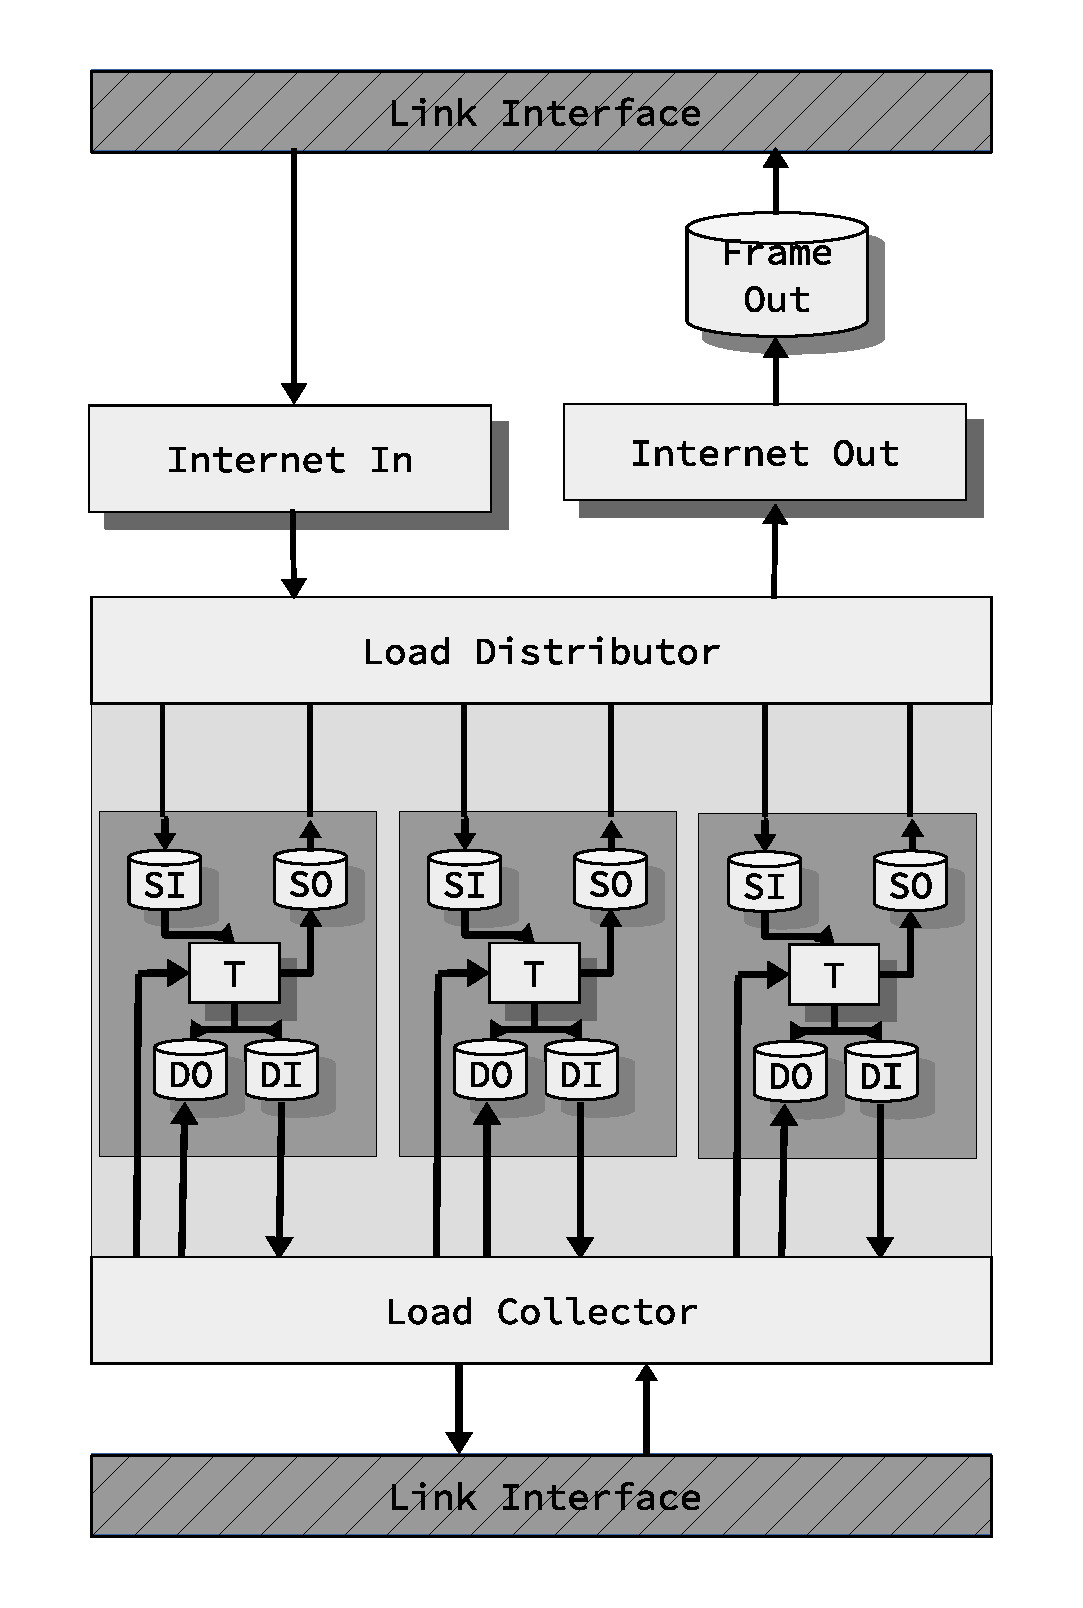
\includegraphics[scale=0.45]{discussion/design_stacked.eps}
\caption{Replicating the "inner" part of the design in order to multiply the
performance. }
\label{fig:design_stacked}
\end{figure}


Even though many optimizations can be done on the network stack codebase
itself, there are other ways of achieving better performance from the project.

\subsection{Increasing the throughput by widening the data channel in the
busses}
Perhaps the most instinctual way of improving the performance of a network
stack is by increasing the throughput. By increasing the width of the
\texttt{data} channel in the buses carrying information, the throughput could
potentially increase manyfold.

While this change is perfectly doable in the hardware and easy to implement in
the code, it might also have some unexpected consequences on the logic of the
processing modules.

For example, while not strictly a requirement, most, if not all, header sizes
are a multiple of 8 bits. By transferring only 1 byte at a time, the system is
sure to never cross the boundary of a header in the same clock cycle. If,
however, the data-bus transferred 2 bytes at a time, the first byte might be
the last part of a header, while the next byte is a data-byte. In that case,
the process has to not only parse the finished header, but also forward the
second byte down to the next process. Here again will the processes need
additional logic needs to check how much of the data-bus actually contains
valid data. Figure \ref{fig:bus_width_boundaries} illustrates the problem of a
data-segment not aligning with the bus-width.

\begin{figure}
\centering
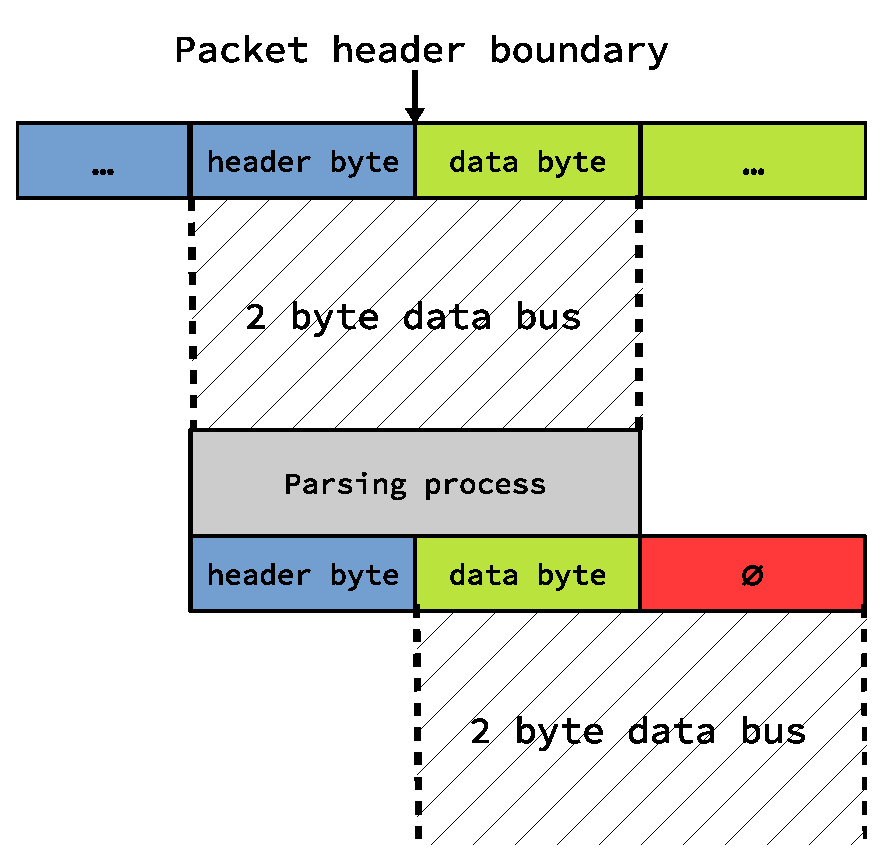
\includegraphics[scale=0.45]{discussion/bus_width_boundaries.eps}
\caption{the design in order to multiply the
performance. }
\label{fig:bus_width_boundaries}
\end{figure}





\subsection{Replicating the system}
During the design-phase, it was important to ensure the active connections
arrived on the same stack, since the IP fragments have to be collected on the
same buffer, and the TCP state has to be synchronized.

The \texttt{Transport} is especially burdensome, as it has to handle both
ingoing- and outgoing-packets, as well as the user interface calls and
protocol-specific handshakes and other operations. Finding a way of getting
around this congestion, it should be possible to parallelize the system for
better performance.

By replicating the networking stack and assign a unique IP address to each, it
should be possible to create a "Load Distributor", distributing the packets
across multiple networking stacks. Figure \ref{fig:design_stacked} shows a
prototype design, where the inner part of the networking stack is duplicated on
the FPGA itself. The \texttt{Load Distributor} conveys the packets to the
appropriate network-stack.

On the other side of the same figure, the \texttt{Load Collector} ensures that
the replicated network stacks work as one, and that they are abstracted away
in the \texttt{User Interface}, so that the user does not have to make up for
the separation. Even though the \texttt{Transport} processes do not share any
information across the stacks, they can have hardcoded \texttt{socket} numbers,
assigning a block of sockets to each stack, so that overlap does not happen.


\section{Usability}
Perhaps the most important aspects of any software project is its usability,
versatility, and its application.
While it is shown in chapter \ref{chap:evaluation} that the networking stack
performs arguably well in a reasonable simulated scenario, it is to be seen
whether the project can bring any value to the user.

\subsection{Intended usage}
The intended usage of the networking stack is to be integrated with existing
FPGA hardware in order add networking capability to a system. These systems
range from simple embedded \gls{iot} devices to large \gls{nic} cards.\\
Although it is possible to connect an SME project with other VHDL projects, it
is much more straight-forward to add the networking code directly into an SME
project.\\
For instance, other SME projects, such as the "High Throughput Image Processing in X-ray
Imaging" developed by Troels Skjøttgaard Ynddal\cite{troels}, which does
real-time image processing on x-ray images, could benefit from a network stack
by sending the processed images to a server for further analysis and backup.

\subsection{Existing solutions}
Sadly, the developed networking stack could not be brought onto an \gls{fpga},
making the comparison to existing solutions difficult.
In theory, if the networking stack worked on an FPGA, it would bring little to
no runtime advantages over existing FPGA TCP/IP stacks, such as the
Xilinx 10Gbps TCP/IP Stack\cite{sidler2016lowlatencytcp}.
However, the networking stack is easily extensible and modular. The design
choices made during the development have proven to make the stack very flexible,
and the programmer can easily add or remove protocols. The use of the C\#
programming language makes it more accessible for software engineers to modify
the code without prior knowledge to the hardware itself, or special \gls{hls}
tools and languages, albeit without the dynamic constructs of the C\# language.


\subsection{Integration with existing hardware}
As an extension to this project, the code for the Digilent Pmod NIC100\cite{pmod_nic100}
has been developed by Carl-Johannes Johnsen to act as the \texttt{Link Interface}
\cite{carl_pmod_nic100}, so that the networking stack could be tested on real
hardware.
While the stack never reached bare-metal, the testing suite simulates this
connection from the Pmod100 into this \texttt{Link Interface}. Although testing
on real hardware has to be carried out for definitive results, the simulation
suggests that this connection with networking hardware can indeed work.


\section{Using C\# with SME}
Not only had the use of C\# with \gls{sme} a great impact on the design, but the
whole project as a whole.

\subsection{Concurrency}
As was the intent of the \gls{sme} project, the messaging framework was
indispensable during the development of the networking stack. Besides not
having to concerns ourselves with the synchronization across processes, the
"Shared Nothing" property of \gls{sme} was a great help during the design, and
forced the design to be neatly isolated in the appropriate layers.

The isolation of each \texttt{Process} object gave a great overview of what each
"thread" of the system was doing. Likewise, the information exchange was very
clear, since it was nicely collected in one place -- the bus.

Sadly, the parsing of network packets is excessively sequential, and the
project does not utilize the full potential of SME in that regard.

\subsection{Cumbersome initialization and alternation}
% Parallelism hard from software
% Initialization of busses is cumbersome
The way projects are written in SME with C\#, the programmer has to
choose a design hardware architecture beforehand, since adding new SME
processes after the fact is cumbersome, and requires a lot of manual
modifications.
For instance, injecting a new process in between two existing processes
requires potentially adding new busses to the system and set these up correctly
in the code. Although this is a trivial task, the process itself is prone to
typos and oversights from the programmer.


\subsection{Using the C\# language}
In the beginning, it was pleasant to use a familiar language for the
implementation of the networking stack. Yet, as the code-base grew in size, the
flaws started to surface.

The C\# programming language is a very actively developed language with many
modern features, it is widely used with a very active community, and it has a lot
of useful packages and frameworks.

When writing code for the simulation, all of these utilities and features can
be used, providing the programmer with endless possibilities for
simulation-scenarios. For instance, inn this system, the simulation processes use the
file-system to load pre-recorded packets and feed them into the
simulation or to create log-files of the simulation\footnote{
A number of experiments have also been carried out in order to replace the
native networking stack with the simulation}.

Unfortunately, almost none of these features are available with \gls{sme}
when writing code for the FPGA, as most of these require dynamic constructs,
such as instantiation of new classes or use of dynamic collections. Although
this restriction is caused by the hardware and not \gls{sme} itself,
the C\# language started to be much less intuitive. Instead of applying
best practices and exploring new features in a well-known and established
language, we had to limit ourselves to the viable subset of the working
features, and create the design around it. While it is understandable why
a proven language is used to test out a new message passing framework,
the C\# language did not always feel right for hardware development, and
the upcoming \gls{smeil} might prove itself to be a welcome addition to
the \gls{sme} project.\cite{github_smeil}.


\subsubsection{Pre-written components and modules}
The \gls{sme} framework already contains premade objects for use, such as the
\texttt{TrueDualPortMemory}, which is a process that helps the programmer write
code interfacing with the built-in block memory on the \gls{fpga}.\\
As of yet, only a few memory components are included in the \gls{sme}
framework.

During development, there was a pattern of prevailing components and systems
reused in multiple processes:
\begin{itemize}
\item \textbf{Generic buffer process}\\
As documented in the design section, the buffers make up a big part of
functionality in the whole system. However, these \gls{fifo} constructs
are very commonly used during FPGA development\cite{fpga_fifo}. A generic
\gls{fifo} buffer component would be a very useful feature during the
development of the networking stack.

\item \textbf{AXI4 communication process}\\
In the processes, the programmer is free to implement any bus interface signal
protocol. Although a custom protocol was implemented for the system, it has
been cumbersome and challenging to implement two processes with a shared signal
protocol. Pre-written processes with support for established signal protocols
could be a valuable addition to the \gls{sme} ecosystem.

\end{itemize}


\subsection{Process state modelling}
Most processes in the system have multiple states, some containing fairly
complex state-transitions, as seen on figure \ref{fig:statemachines_internetin_transport}
in chapter \ref{chap:implementation}.\\
Introduced in the implementation chapter, \gls{sme} provides the
\texttt{StateProcess} class to simplify the creation of processes with
multiple states. This class proved itself to be immensely helpful in the
\texttt{Internet Out} process, which consist solely of sequential states.
Unfortunately, this construct is inadequate and incomplete to model the rest of
the computing processes, which were slightly more complex state-machines, as
those used in the system.

\subsubsection{Repeated code}
\begin{figure}
\centering
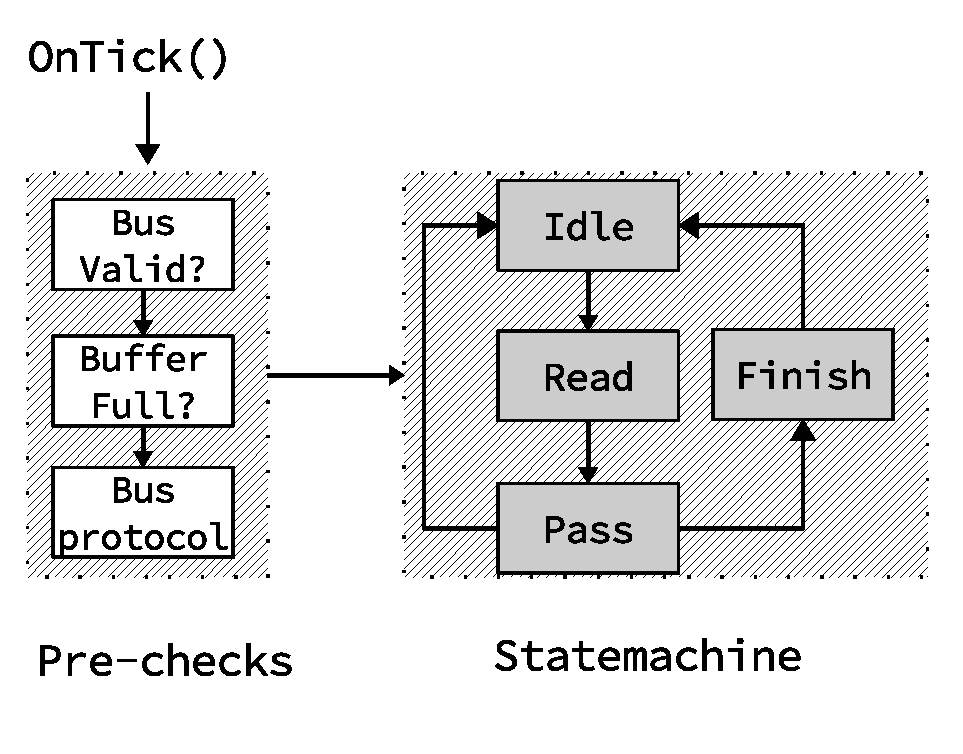
\includegraphics[scale=0.45]{discussion/fsm_prestates.eps}
\caption{An example of a process state-machine with pre-checks regardless of
the current state.}
\label{fig:fsm_prestates}
\end{figure}

The first identified issue was that most processes need to run certain checks on the
start of each clock cycle, such as checking the validity of the busses,
ensuring that there were no errors in the data-stream, maintain a bus signal
protocol, or make sure that some other limitations are met.
With the conventional \texttt{StateMachine}, this is intricate to write these
checks without much repetition. Instead, in this project, regular processes are
used in combination with an internal variable keeping track of the state.
This subtle difference lets the programmer have a unified entry-point to the
code, and branching code can be written to enter the appropriate
state-functions in the code.
For instance, figure \ref{fig:fsm_prestates} visualizes that a unified
pre-checks can be run prior to enter state-specific code. This adds a lot to
the length of the "code-path", but it avoids a lot of repetition in the code.


\subsubsection{Complicated state changes}\notejan{Spoerg Carl om hans kommentar}
Another common issue with modelling state-machines with \gls{sme} was certain
state-changes. In situations where a process is executing the last cycle of a
state that writes to some bus, a state-change is often desired in the end.
However, most state-transitions need to do some cleanup, for instance resetting
variables or re-initialize busses. If this cleanup happens in the same clock as
the last byte is written to the bus, this value will never arrive at the other
end. To circumvent this, the \texttt{Finish} state was utilized, which delays
the state-transition a single clock, giving the busses a clock-cycle window to
propagate correctly.

While this solution worked fine, the code itself was identical across processes
with this issue, and re-implementing was cumbersome and error-prone.

\subsection{Bugs and other lesser issues}
The\gls{sme} framework has been surprisingly stable, albeit with a few minor
bugs. Although most of these issues are being fixed at the time of writing,
they were still a noticeable hindrance during development:
\begin{itemize}
\item \textbf{Reserved VHDL keywords}\\
Certain words in the C\# code were reserved in\gls{vhdl}. While this is a
non-issue if the project is not being compiled to \gls{vhdl} code, this needed
to be taken into consideration during development. One such reserved word  was
the "Transport", used to denote the \texttt{Transport} process class.

\item \textbf{C\# structs}\\
A lot of information has to be passed between the buffers and processes. For
the sake of readability and maintainability of the codebase, this data is best
encapsulated in namespaces for a hierarchical organization.
Luckily, \texttt{struct}s became available shortly after the discovery of this
requirement, and are used in the project. For instance, the
\texttt{InterfaceBus} uses two of the \texttt{InterfaceData} struct.

\item \textbf{Slow simulation}\notejan{Naevn at det stadig kan vaere hurtigere
	end VHDL}\\
The tests carried out during the evaluation of the system were astonishingly
slow. While the simulation ran at an acceptable rate in the beginning, it
started slowing down as the test progressed. A simulation lasting multiple
hours only managed to simulate a few millions of clock-cycles.

\end{itemize}


